\subsection{Recap: Process Models}
\begin{frame}{\inserttitle}
	\lectureseriesoverview[8]
\end{frame}

\begin{frame}{\myframetitle\ \deutschertitel{Vorgehensmodelle}}
	\begin{definition}{Recap: The Software Life Cycle}
		\waterfallcartoon
	\end{definition}

	\uncover<2->{\begin{mycolumns}[animation=none]
		\begin{example}{Process Models for Single-System Engineering}
			waterfall model, V model, scrum, \ldots
		\end{example}
	\mynextcolumn
		\uncover<3->{\begin{note}{Process Models for Product-Line Engineering}
			???
		\end{note}}
	\end{mycolumns}}
\end{frame}

\subsection{Domain and Application Engineering}
\begin{frame}{\myframetitle}
	\begin{note}{A Process Model for Product-Line Engineering}
		idea: split development into two phases, one for product line and one for products
	\end{note}
	\begin{mycolumns}[animation=none,T]
		\uncover<2->{\begin{definition}{Domain Engineering\mysource{\fospl\mypages{21--22}}}
			\mycite{\emph{Domain engineering} is the process of analyzing the domain of a product line and developing reusable artifacts.}
		\end{definition}
		\begin{note}{Domain Engineering\mysource{\fospl\mypage{21}}}
			\begin{itemize}
				\item development for reuse
				\item prepares artifacts to be used in products (or during application engineering)
				\item goal: reduce effort per product (i.e., effort during application engineering)
			\end{itemize}
		\end{note}}
	\mynextcolumn
		\uncover<3->{\begin{definition}{Application Engineering\mysource{\fospl\mypage{21}}}
			\mycite{\emph{Application engineering} has the goal of developing a specific product for the needs of a particular customer (or other stakeholder).}
		\end{definition}
		\begin{note}{Application Engineering\mysource{\fospl\mypage{21}}}
			\begin{itemize}
				\item development with reuse
				\item build products using artifacts from domain engineering
				\item repeated for every product
				\item \mycite{application} of the product line (i.e., suitable for application and system software)
			\end{itemize}
		\end{note}}
	\end{mycolumns}
\end{frame}

%\begin{frame}{\myframetitle}
%	\begin{mycolumns}
%		\mydefinition{Product-Line Engineering\mysource{\sple\mypage{14}}}{
%			\mycite{\emph{Software product-line engineering} is a paradigm to develop software applications (software-intensive systems and software products) using software platforms and mass customization.}
%		}
%	\mynextcolumn
%	\end{mycolumns}
%\end{frame}

\begin{frame}{Recap: Domain}
	\begin{mycolumns}[animation=none]
		\begin{definition}{Recap: Domain \deutsch{Domäne} \hfill\tiny\lectureintroduction}
			\mycitebegin A \emph{domain} is an area of knowledge that:
			\begin{itemize}
				\item is scoped to maximize the satisfaction of the requirements of its stakeholders,
				\item includes a set of concepts and terminology understood by practitioners in that area,
				\item and includes the knowledge of how to build software systems (or parts of
				software systems) in that area.\myciteend
			\end{itemize}
		\end{definition}
	\mynextcolumn
	\end{mycolumns}
\end{frame}
% TODO introduce domain and application artifacts here? see \sple
% would also apply to domain/application requirements, but domain requirement is a confusing term (as it would refer to requirements of a product line and not all of a domain)

% terms used in the remained are mostly taken from \sple and some from \fospl

\begin{frame}%{\myframetitle}
	\footnotesize%
	\begin{mycolumns}[columns=3,widths={10,70,10},animation=none]
		\renewcommand{\projectcartoonwidth}{1}\hprojectcartoon{01}{Product-Line Requirements}
	\mynextcolumn
		\begin{note}{Domain Engineering}
			\renewcommand{\projectcartoonwidth}{.15}%
			\hprojectcartoon{02}{Domain Analysis}%
			\hprojectcartoon{03}{Domain Design}%
			\hprojectcartoon{04}{Domain Implementation}%
			\hprojectcartoon{05}{Domain Testing}
		\end{note}
	\mynextcolumn
	\end{mycolumns}
	\pause
	\begin{mycolumns}[columns=3,widths={10,70,10},animation=none]
		\renewcommand{\projectcartoonwidth}{1}\projectcartoon{01}{Product Requirements}
	\mynextcolumn
		\begin{note}{Application Engineering}
			\renewcommand{\projectcartoonwidth}{.15}%
			\projectcartoon{02}{Application Analysis}%
			\projectcartoon{03}{Application Design}%
			\projectcartoon{04}{Application Implementation}%
			\projectcartoon{05}{Application Testing}
		\end{note}
	\mynextcolumn
		\renewcommand{\projectcartoonwidth}{1}\projectcartoon{13}{Product}
	\end{mycolumns}
\end{frame}

\subsection{Analysis and Design}
\begin{frame}{Domain and Application Analysis}\small
	\begin{mycolumns}[T,columns=3,widths={10}]
		\renewcommand{\projectcartoonwidth}{1}\hprojectcartoon{02}{}
	\mynextcolumn
		\begin{definition}{Domain Analysis\mysource{\fospl\mypage{21}, \sple\mypage{25}}}
			\begin{itemize}
				\item requirements analysis for a product line
				\item define scope of the product line
				\item which features are in scope?
				\item which combinations of features are in scope?
				\item typically results in a feature model and features mapped to requirements
			\end{itemize}
		\end{definition}
		\begin{definition}{Domain Scoping\mysource{\fospl\mypage{22}}}
			which requirements of a domain are in scope for the product line?
			\begin{itemize}
				\item domain experts collect requirements (e.g., from existing systems, interviews, potential customers)
				\item often economical decision by managers
			\end{itemize}
		\end{definition}
		% TODO introduce term Domain Modeling?
	\mynextcolumn
		\begin{definition}{Application Analysis\mysource{\fospl\mypages{21--25}}}
			\begin{itemize}
				\item requirements analysis for a product
				\item based on the output of domain analysis
				\item ideally: customer requirements mapped to a feature selection
				\item alternative strategies for new and unsupported requirements:
					\begin{enumerate}\small % TODO Benno: why is the font size changed here?
						\item requirement is out of scope (i.e., no product made available)
						\item document for custom development (i.e., development in application engineering)
						\item integrate into domain analysis (i.e., development in domain engineering)
					\end{enumerate}
				\item best strategy depends on the situation
			\end{itemize}
		\end{definition}
		% TODO pointer to staged configuration? or even introduce it here?
	\end{mycolumns}
\end{frame}
% TODO running example

\begin{frame}{Domain Scoping in Practice}
	\centering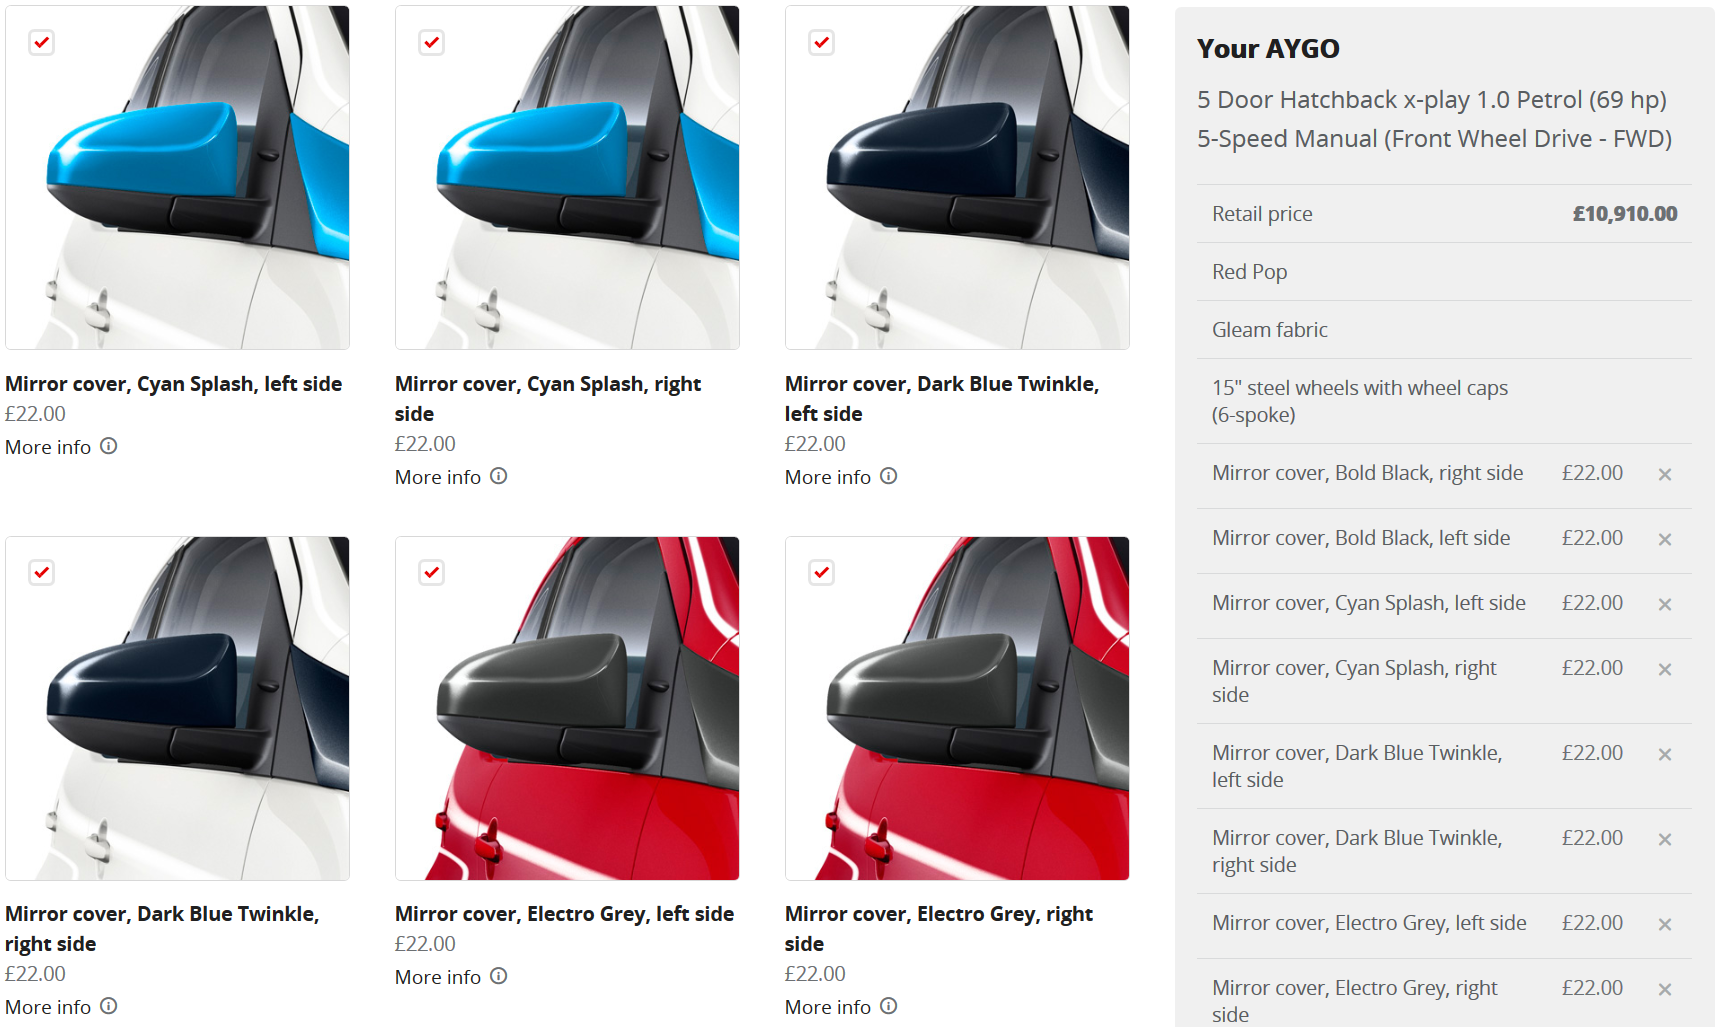
\includegraphics[width=.8\linewidth]{toyota-aygo-mirrorcovers}
\end{frame}
% TODO note what we see here

\begin{frame}{Domain and Application Design}
	\begin{mycolumns}[T,columns=3,widths={10}]
		\renewcommand{\projectcartoonwidth}{1}\hprojectcartoon{03}{}
	\mynextcolumn
		\begin{definition}{Domain Design\mysource{\sple\mypage{26}}} % TODO see \sple Chapter 6+11
			\begin{itemize}
				\item development of a reference architecture (e.g., client-server or pipe-and-filter)
				\item common, high-level structure for all products
				\item decision on implementation technique
			\end{itemize}
		\end{definition}
	\mynextcolumn
		\begin{definition}{Application Design\mysource{\sple\mypages{32--33}}}
			\begin{itemize}
				\item create application architecture
				\item derived from reference architecture
				\item based on feature selection
				\item design decisions for application-specific requirements
			\end{itemize}
		\end{definition}
	\end{mycolumns}
\end{frame}

\subsection{Implementation and Testing}
\begin{frame}{Domain and Application Implementation}
	\begin{mycolumns}[T,columns=3,widths={10}]
		\renewcommand{\projectcartoonwidth}{1}\hprojectcartoon{04}{}
	\mynextcolumn
		\begin{definition}{Domain Implementation\mysource{\fospl\mypage{21}}} % TODO see \sple Chapter 7+12
			\begin{itemize}
				\item development of reusable artifacts
				\item implementation of features identified during domain analysis
				\item implementation largely depends on the implementation technique chosen in domain design
			\end{itemize}
		\end{definition}
	\mynextcolumn
		\begin{definition}{Application Implementation\mysource{\fospl\mypage{21}}}
			\begin{itemize}
				\item development of products based on reusable artifacts
				\item ideally: fully automated generation (aka.\ \emph{product derivation})
				\item full automation not feasible \ldots
					\begin{enumerate}
						\item when custom development is needed (i.e., for application-specific requirements)
						\item for clone-and-own, components, services
					\end{enumerate}
			\end{itemize}
		\end{definition}
	\end{mycolumns}
\end{frame}
% reusable parts indespensible, reusable architecture optional
% fully automatic or semi-automatic with custom design and implementation

\begin{frame}{Domain and Application Testing}
	\begin{mycolumns}[T,columns=3,widths={10}]
		\renewcommand{\projectcartoonwidth}{1}\hprojectcartoon{05}{}
	\mynextcolumn
		\begin{definition}{Domain Testing\mysource{\sple\mypage{27}}} % TODO see \sple Chapter 8+13
			\begin{itemize}
				\item validation and verification of reusable artifacts
				\item development of reusable tests
				\item testing of features in isolation, if possible \lectureanalyses
				\item testing of sample products \lecturetesting
			\end{itemize}
		\end{definition}
	\mynextcolumn
		\begin{definition}{Application Testing\mysource{\sple\mypages{33--34}}}
			\begin{itemize}
				\item testing of the application
				\item reuse of test artifacts from domain testing
				\item new test artifacts for custom development
			\end{itemize}
		\end{definition}
	\end{mycolumns}
\end{frame}
% systematic testing, sometimes skipped (e.g., if product derivation not automatic)
% testing of a single product, sometimes optional

\subsection{Problem and Solution Space}
\begin{frame}{\myframetitle}
	\begin{mycolumns}[widths={35},T]
		\begin{definition}{Problem Space\mysource{\fospl\mypage{21}}}
			\mycite{The \emph{problem space} takes the perspective of stakeholders and their problems, requirements, and views of the entire domain and individual products. Features are, in fact, domain abstractions that characterize the problem space.}
		\end{definition}
		{\small\featureDiagram{Graph,abstract[Directed,optional,concrete][Weighted,optional,concrete][OptimalConnection,optional,concrete]}}
		
		\centering
		\pic[width=.4\linewidth]{preprocessor-wilderness-problem-space}
	\mynextcolumn
		\begin{definition}{Solution Space\mysource{\fospl\mypage{21}}}
			\mycite{The \emph{solution space} represents the developer’s and vendor’s perspectives. It is characterized by the terminology of the developer, which includes names of functions, classes, and program parameters. The solution space covers the design, implementation, and validation and verification of features and their combinations in suitable ways to facilitate systematic reuse.}
		\end{definition}
		\centering
		\pic[width=.6\linewidth,trim=20 20 20 40,clip]{preprocessor-wilderness-solution-space}
	\end{mycolumns}
\end{frame}
% TODO move to the beginning of this lecture?

\subsection{Overview on Domain and Application Engineering}
\begin{frame}%{\myframetitle}
	\footnotesize%
	\begin{mycolumns}[columns=3,widths={10,70,10},animation=none]
		\renewcommand{\projectcartoonwidth}{1}\hprojectcartoon{01}{Product-Line Requirements}
	\mynextcolumn
		\begin{note}{Domain Engineering}
			\renewcommand{\projectcartoonwidth}{.15}%
			\hprojectcartoon{02}{Domain Analysis}%
			\hprojectcartoon{03}{Domain Design}%
			\hprojectcartoon{04}{Domain Implementation}%
			\hprojectcartoon{05}{Domain Testing}
		\end{note}
	\mynextcolumn
	\end{mycolumns}
	\pause
	\begin{mycolumns}[columns=3,widths={10,70,10},animation=none]
		\renewcommand{\projectcartoonwidth}{1}\projectcartoon{01}{Product Requirements}
	\mynextcolumn
		\begin{note}{Application Engineering}
			\renewcommand{\projectcartoonwidth}{.15}%
			\projectcartoon{02}{Application Analysis}%
			\projectcartoon{03}{Application Design}%
			\projectcartoon{04}{Application Implementation}%
			\projectcartoon{05}{Application Testing}
		\end{note}
	\mynextcolumn
		\renewcommand{\projectcartoonwidth}{1}\projectcartoon{13}{Product}
	\end{mycolumns}
\end{frame}
% lecture 8: show how linux in lecture 4+5 relates to problem space (kconfig)/mapping (kbuild)/solution space (cpp) - put this into the four-quadrant model

% TODO visual summary, including pictures from earlier lectures and references to lectures